\chapter{Derivatives of Common Functions}
%Begin Section 2.1
\section{Inverse Functions}
The derivatives calculated in the previous chapter were mostly for polynomials
and a few trigonometric functions. This chapter will show how to find the
derivatives of other types of functions, beginning in this section with inverse
functions. The idea here is that if a function is differentiable and has
an inverse then that inverse function is also differentiable.

\piccaption[]{\label{fig:function}}\parpic[r]{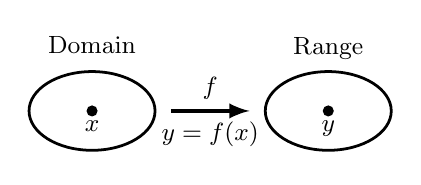
\begin{tikzpicture}[every node/.style={font=\small}]
 \draw [line width=1pt] (0,0) ellipse (0.8 and 0.5);
 \fill (0,0) circle (2pt);
 \node [below] at (0,0) {$x$};
 \node [above] at (0,0.6) {Domain};
 \draw [line width=1pt] (3,0) ellipse (0.8 and 0.5);
 \fill (3,0) circle (2pt);
 \node [below] at (3,0) {$y$};
 \node [above] at (3,0.53) {Range};
 \draw [-latex,line width=1.5pt] (1,0) -- (2,0) node[midway,above] {$f$}
  node[midway,below] {$y=f(x)$};
\end{tikzpicture}}
Recall that a \textbf{function}\index{function} is a rule that assigns a single
object $y$ from one set (the \textbf{range})\index{range} to each object $x$
from another set (the \textbf{domain}).\index{domain} That rule can be written
as $y = f(x)$, where $f$ is the function (see Figure \ref{fig:function}). There
is a simple \emph{vertical rule} for determining whether a rule $y=f(x)$ is a
function: $f$ is a function if and only if every vertical line intersects the
graph of $y=f(x)$ in the $xy$-coordinate plane at most once (see
Figure \ref{fig:verticalrule}).

\begin{figure}[h]
 \centering
 \subfloat[][ $f$ is a function]{
  \begin{tikzpicture}[>=latex,every node/.style={font=\small}]
   \draw[<->,black!60,line width=1pt] (0,2) node[above] {$y$} |- (4,0) node[right] {$x$};
   \draw [linecolor,line width=1.5pt] (0.5,0.5) parabola[bend at end] (3.5,1.5);
   \node[above] at (3.5,1.5) {$y=f(x)$};
   \draw[line width=1pt] (1.5,0.5) -- (1.5,2);
  \end{tikzpicture}}
 \qquad\qquad
 \subfloat[][ $f$ is not a function]{
  \begin{tikzpicture}[>=latex,every node/.style={font=\small}]
   \draw[<->,black!60,line width=1pt] (0,2) node[above] {$y$} |- (4,0) node[right] {$x$};
   \draw [linecolor,line width=1.5pt] (0.5,1.5) parabola bend  (3.5,1) (2.5,0.5);
   \node[above] at (1.5,1.5) {$y=f(x)$};
   \draw[line width=1pt] (2.8,0.2) -- (2.8,2);
  \end{tikzpicture}}\vspace{-2mm}
 \caption[]{\quad Vertical rule for functions}
 \label{fig:verticalrule}
\end{figure}

Recall that a function $f$ is \textbf{one-to-one}\index{one-to-one} (often
written as $1-1$) if it assigns distinct values of $y$ to distinct values of
$x$. In other words, if $x_1 \ne x_2$ then $f(x_1 ) \ne f(x_2 )$. Equivalently,
$f$ is one-to-one if $f(x_1 ) = f(x_2 )$ implies $x_1 = x_2$. There is a simple
\emph{horizontal rule} for determining whether a function $y=f(x)$ is
one-to-one: $f$ is one-to-one if and only if every horizontal line intersects
the graph of $y=f(x)$ in the $xy$-coordinate plane at most once (see
Figure \ref{fig:horizontalrule}).
\newpage
\begin{figure}[h]
 \centering
 \subfloat[][ $f$ is one-to-one]{
  \begin{tikzpicture}[every node/.style={font=\small}]
   \draw[latex-latex,black!60,line width=1pt] (0,2) node[above] {$y$} |- (4,0) node[right] {$x$};
   \draw [linecolor,line width=1.5pt] (0.5,0.5) parabola[bend at end] (3.5,1.5);
   \node[above] at (3.5,1.5) {$y=f(x)$};
   \draw[line width=1pt] (0.5,1) -- (2.5,1);
  \end{tikzpicture}}
 \qquad\qquad
 \subfloat[][ $f$ is not one-to-one]{
  \begin{tikzpicture}[every node/.style={font=\small}]
   \draw[latex-latex,black!60,line width=1pt] (0,2) node[above] {$y$} |- (4,0) node[right] {$x$};
   \draw [linecolor,line width=1.5pt] (0.5,0.5) parabola bend  (2,1.5) (3.5,0.5);
   \node[above] at (2,1.5) {$y=f(x)$};
   \draw[line width=1pt] (0.5,1) -- (3.5,1);
  \end{tikzpicture}}\vspace{-2mm}
 \caption[]{\quad Horizontal rule for one-to-one functions}
 \label{fig:horizontalrule}
\end{figure}

If a function $f$ is one-to-one on its domain, then $f$ has an
\textbf{inverse function}, denoted by $f^{-1}$, such that $y=f(x)$ if and only
if $f^{-1}(y) = x$. The domain of $f^{-1}$ is the range of
$f$.\index{inverse function}\index{function!inverse}

The basic idea is that $f^{-1}$ ``undoes'' what $f$ does, and vice versa. In
other words,
\begin{alignat*}{3}
 f^{-1}(f(x)) ~&=~ x \quad&&\text{for all $x$ in the domain of $f$, and}\\
 f(f^{-1}(y)) ~&=~ y \quad&&\text{for all $y$ in the range of $f$.}
\end{alignat*}

Intuitively it is clear that a function is one-to-one (and hence invertible)
when it is either strictly increasing or strictly decreasing; if the function,
say, increases and then decreases (as in Figure \ref{fig:horizontalrule}(b))
then the horizontal rule would be violated around that ``turning point.'' For
differentiable functions a positive derivative means the function is increasing,
while a negative derivative means the function is decreasing (this will be
proved in Chapter 3).

However, a function can still be one-to-one even if
its derivative is zero only at isolated points (i.e. not identically zero over
an entire interval of points) and either positive everywhere else or negative
everywhere else. For example, the function $f(x) = x^3$ has derivative
$f'(x) = 3x^2$, which is zero only at the isolated point $x = 0$ and positive
for all other values of $x$. Clearly $f$ is one-to-one over the set of all real
numbers (why?) and hence it has an inverse function $x = f^{-1}(y) = \sqrt[3]{y}$
defined for all real numbers $y$ (i.e. the range of $f$).

Thus, having a derivative that is either
always positive or always negative is \emph{sufficient} for a function to be
one-to-one but not \emph{necessary}. Having a nonzero derivative is necessary,
though, for the inverse function to be differentiable.

In algebra you learned that $\frac{a}{b} = \frac{1}{\frac{b}{a}}$ for all real
numbers $a \ne 0$ and $b \ne 0$ (and hence $\frac{b}{a} \ne 0$). The same holds
true for the infinitesimals $\dy$ and $\dx$ (nonzero by definition) since they
can be treated like numbers, which immediately yields a formula for the
derivative of an inverse function:

\statethm{thm:invderiv}{\textbf{Derivative of an Inverse Function:} If $y = f(x)$
is differentiable and has an inverse function $x = f^{-1}(y)$, then $f^{-1}$ is
differentiable and its derivative is
\[
 \dxdy ~=~ \frac{1}{\dydx} \qquad\text{if $~\dydx \ne 0$.}
\]}
The inverse of a function would still exist at a point where $\dydx = 0$
but it would not be differentiable there, since its derivative would be the
undefined quantity $\frac{1}{0}$.

Since $y$ is a function of $x$, $\dydx$ will be in terms of $x$ and hence
$\frac{1}{\dydx}$ will be in terms of $x$. However, since (by invertibility)
$x$ is a function of $y$, $\dxdy$ would normally be in terms of $y$, not $x$,
so that the two sides of the equation $\dxdy = \frac{1}{\dydx}$ are not in the
same terms!
One way to handle this discrepancy is to use the formula $y = f(x)$ to solve for
$x$ in terms of $y$ then substitute that expression into $\dydx$, so that
$\dxdy = \frac{1}{\dydx}$ is now in terms of $y$. That might not always be
possible, however (e.g. try solving for $x$ in the formula $y = x \sin x$).

\begin{exmp}\label{exmp:invderiv}
 Find the inverse $f^{-1}$ of the function $f(x) = x^3$ then find the derivative
 of $f^{-1}$.\vspace{1mm}
 \par\noindent\emph{Solution:} The function $y = f(x) = x^3$ is one-to-one over
 the set of all real numbers (why?) so it has an inverse function $x = f^{-1}(y)$
 defined for all real numbers, namely $x = f^{-1}(y) = \sqrt[3]{y}$.\vspace{1mm}
 
 \par\noindent The derivative of $f^{-1}$ is
 \begin{align*}
  \dxdy ~&=~ \frac{1}{\dydx} ~=~ \frac{1}{3x^2} \quad\text{, which is in terms of $x$,
             so putting it in terms of $y$ yields}\\[6pt]
         &=~ \frac{1}{3 \left(\sqrt[3]{y}\right)^2} ~=~
		     \frac{1}{3 y^{2/3}}
 \end{align*}
 which agrees with the derivative obtained by differentiating $x = \sqrt[3]{y}$
 directly. Note that this derivative is defined for all $y$ except $y = 0$,
 which occurs when $x = \sqrt[3]{0} = 0$, i.e. at the point $(x,y) = (0,0)$.
\end{exmp}
\divider
\vspace{3mm}

Functions are often expressed in terms of $x$, so it is common to see an
inverse function also expressed in terms of $x$: writing the inverse
of $f(x) = x^3$ as $f^{-1}(x) = \sqrt[3]{x}$ (not as
$f^{-1}(y) = \sqrt[3]{y}$)), as confusing as that might be. In that case, the
idea is to switch the roles of $x$ and $y$ in the original function $y = f(x)$,
making it $x = f(y)$, and then write $y = f^{-1}(x)$ and use
\[
 \dydx ~=~ \frac{1}{\dxdy}
\]
to put the derivative of $f^{-1}$ in terms of $x$, following the same procedure
mentioned earlier.

\begin{exmp}\label{exmp:invderivalt}
 Find the inverse $f^{-1}$ of the function $f(x) = x^3$ then find the derivative
 of $f^{-1}$.\vspace{1mm}
 \par\noindent\emph{Solution:} Rewrite $y = f(x) = x^3$ as
 $x = f(y) = y^3$, so that its inverse function $y = f^{-1}(x)= \sqrt[3]{x} $
 has derivative
 \begin{align*}
  \dydx ~&=~ \frac{1}{\dxdy} ~=~ \frac{1}{3y^2} \quad\text{, which is in terms of $y$,
             so putting it in terms of $x$ yields}\\[6pt]
         &=~ \frac{1}{3 \left(\sqrt[3]{x}\right)^2} ~=~
		     \frac{1}{3 x^{2/3}}
 \end{align*}
 which agrees with the derivative obtained by differentiating $y = \sqrt[3]{x}$
 directly.
\end{exmp}
\divider
\newpage
To obtain a formula in prime notation for the derivative of an inverse function,
notice that for all $x$ in the domain of an invertible differentiable function
$f$,
\[
 f^{-1}(f(x)) ~=~ x \quad\Rightarrow\quad
 \ddx\,\left(f^{-1}(f(x))\right) ~=~ \ddx\,(x) \quad\Rightarrow\quad
 \left(f^{-1}\right)'(f(x)) \;\cdot\; f'(x) ~=~ 1
\]
by the Chain Rule, and hence:

\statethm{thm:invprime}{\vspace{-5mm}\begin{align*}
 \left(f^{-1}\right)'(f(x)) ~&=~ \frac{1}{f'(x)} \qquad\text{if $~f'(x) \ne 0$}
\intertext{Two equivalent ways to write this are:}
 \left(f^{-1}\right)'(c) ~&=~ \frac{1}{f'(a)} \qquad\text{where $c = f(a)$ and $~f'(a) \ne 0$}
\intertext{and}
 \left(f^{-1}\right)'(x) ~&=~ \frac{1}{f'(f^{-1}(x))} \qquad\text{if $~f'(f^{-1}(x)) \ne 0$}
\end{align*}}
\divider
\vspace{3mm}
\startexercises\label{sec2dot1}
{\small
\probs{A}
\par\noindent For Exercises 1-8, show that the given function $y = f(x)$ is
 one-to-one over the given interval, then find the formulas for the inverse
 function $f^{-1}$ and its derivative. Use Example \ref{exmp:invderivalt} as a
 guide, including putting $f^{-1}$ and its derivative in terms of $x$.
\begin{enumerate}[\bfseries 1.]
 \begin{multicols}{2}
  \item $f(x) = x$, for all $x$
  \item $f(x) = 3x$, for all $x$
 \end{multicols}
 \begin{multicols}{2}
  \item $f(x) = x^2$, for all $x \ge 0$
  \item $f(x) = \sqrt{x}$, for all $x \ge 0$
 \end{multicols}
 \begin{multicols}{2}
  \item $f(x) = \frac{1}{x}$, for all $x > 0$
  \item $f(x) = \frac{1}{x}$, for all $x < 0$
 \end{multicols}
 \begin{multicols}{2}
  \item $f(x) = \frac{1}{x^2}$, for all $x > 0$
  \item $f(x) = x^5$, for all $x\vphantom{\frac{1}{x^2}}$
 \end{multicols}
 \item The unit circle $x^2 + y^2 = 1$ does not define $y$ as a single function
  of $x$, since $y = \pm \sqrt{1 - x^2}$ defines two separate functions. But
  the part of the unit circle in the first quadrant, i.e. for $0 \le x \le 1$
  and $0 \le y \le 1$, does define $y = f(x) = \sqrt{1 - x^2}$ as a single
  function of $x$ that is one-to-one on the interval $\ival{0}{1}$. Find the
  formulas for its inverse function $f^{-1}$ and its derivative.
\suspend{enumerate}
\probs{B}
\resume{enumerate}[{[\bfseries 1.]}]
 \item Show that if $f$ is differentiable and invertible, and if $f^{-1}$ is
  twice-differentiable, then
  \begin{displaymath}
   \left(f^{-1}\right)''(x) ~=~ -\frac{f''(f^{-1}(x))}{\left(f'(f^{-1}(x))\right)^3} ~.
  \end{displaymath}
\end{enumerate}}
\newpage
%Begin Section 2.2
\section{Trigonometric Functions and Their Inverses}
The graphs of the six trigonometric functions are shown in Figure
\ref{fig:trigfcns}:

\begin{figure}[ht]
 \centering
 \subfloat[][ $y\;=\;\sin\,x$]{
  \begin{tikzpicture}[scale=1.2,every node/.style={font=\small}]
  \begin{scope}[shift={(0,0)},color=linecolor,line width=1.5pt,x=3cm/360]
  \pgfplothandlerlineto
  \pgfplotfunction{\x}{0,5,...,360}{\pgfpointxy{\x}{sin(\x)}}
  \pgfusepath{stroke}
  \draw[black!60,line width=1pt,-latex] (0,0) -- (400,0) node[right] {$x$};
  \draw[black!60,line width=1pt,-latex] (0,-1.2) -- (0,1.4) node[above] {$y$};
  \node[black,left] at (0,0) {$0$};
  \foreach \pos in {90,180,270,360}
   \draw[black!60,line width=0.3pt,shift={(\pos,0)}] (0pt,3pt) -- (0pt,-3pt);
  \foreach \pos in {-1,1}
   \draw[black!60,line width=0.3pt,shift={(0,\pos)}] (3pt,0pt) -- (-3pt,0pt);
  \node[black,left] at (0,1) {$1$};
  \node[black,left] at (0,-1) {$-1$};
  \node[black,below] at (90,-0.1) {$\tfrac{\pi}{2}$};
  \node[black,below] at (180,-0.1) {$\pi$};
  \node[black,below] at (270,-0.1) {$\tfrac{3\pi}{2}$};
  \node[black,below] at (368,-0.1) {$2\pi$};
 \end{scope}
\end{tikzpicture}}
 \quad
 \subfloat[][ $y\;=\;\cos\,x$]{
  \begin{tikzpicture}[scale=1.2,every node/.style={font=\small}]
  \begin{scope}[shift={(0,0)},color=linecolor,line width=1.5pt,x=3cm/360]
  \pgfplothandlerlineto
  \pgfplotfunction{\x}{0,5,...,360}{\pgfpointxy{\x}{cos(\x)}}
  \pgfusepath{stroke}
  \draw[black!60,line width=1pt,-latex] (0,0) -- (400,0) node[right] {$x$};
  \draw[black!60,line width=1pt,-latex] (0,-1.2) -- (0,1.4) node[above] {$y$};
  \node[black,left] at (0,0) {$0$};
  \foreach \pos in {90,180,270,360}
   \draw[black!60,line width=0.3pt,shift={(\pos,0)}] (0pt,3pt) -- (0pt,-3pt);
  \foreach \pos in {-1,1}
   \draw[black!60,line width=0.3pt,shift={(0,\pos)}] (3pt,0pt) -- (-3pt,0pt);
  \node[black,left] at (0,1) {$1$};
  \node[black,left] at (0,-1) {$-1$};
  \node[black,below] at (90,-0.1) {$\tfrac{\pi}{2}$};
  \node[black,below] at (180,-0.1) {$\pi$};
  \node[black,below] at (275,-0.1) {$\tfrac{3\pi}{2}$};
  \node[black,below] at (362,-0.1) {$2\pi$};
 \end{scope}
\end{tikzpicture}}
 \quad
 \subfloat[][ $y\;=\;\tan\,x$]{
  \begin{tikzpicture}[scale=1.2,every node/.style={font=\small}]
  \begin{scope}[shift={(0,0)},color=linecolor,line width=1.5pt,x=3cm/360]
  \pgfplothandlerlineto
  \pgfplotfunction{\x}{-82,-80,...,82}{\pgfpointxy{\x}{0.34*tan(0.9*\x)}}
  \pgfusepath{stroke}
  \draw[black!60,dashed,line width=0.3pt] (-90,-1.2) -- (-90,1.2);
  \draw[black!60,dashed,line width=0.3pt] (90,-1.2) -- (90,1.2);
  \draw[black!60,line width=1pt,-latex] (-130,0) -- (130,0) node[right] {$x$};
  \draw[black!60,line width=1pt,-latex] (0,-1.2) -- (0,1.4) node[above] {$y$};
  \node[black,below right] at (0,0) {$0$};
  \node[black,below left] at (-90,-0.1) {$-\tfrac{\pi}{2}$};
  \node[black,below right] at (90,-0.1) {$\tfrac{\pi}{2}$};
 \end{scope}
\end{tikzpicture}}
\\\vspace{1mm}
 \subfloat[][ $y~=~\csc\,x$]{
  \begin{tikzpicture}[scale=1.2,every node/.style={font=\small}]
  \begin{scope}[shift={(0,0)},color=linecolor,line width=1.5pt,x=3cm/360]
  \pgfplothandlerlineto
  \pgfplotfunction{\x}{8,10,...,172}{\pgfpointxy{\x}{0.5 + 0.1/sin(\x)}}
  \pgfusepath{stroke}
  \pgfplothandlerlineto
  \pgfplotfunction{\x}{188,190,...,352}{\pgfpointxy{\x}{-0.5 + 0.1/sin(\x)}}
  \pgfusepath{stroke}
  \draw[black!60,line width=1pt,-latex] (0,0) -- (400,0) node[right] {$x$};
  \draw[black!60,line width=1pt,-latex] (0,-1.2) -- (0,1.5) node[above] {$y$};
  \draw[black!60,dashed,line width=0.3pt] (180,-1.2) -- (180,1.4);
  \draw[black!60,dashed,line width=0.3pt] (360,-1.2) -- (360,1.4);
  \node[black,left] at (0,0) {$0$};
  \foreach \pos in {90,180,270,360}
   \draw[black!60,line width=0.3pt,shift={(\pos,0)}] (0pt,3pt) -- (0pt,-3pt);
  \foreach \pos in {-0.6,0.6}
   \draw[black!60,line width=0.3pt,shift={(0,\pos)}] (3pt,0pt) -- (-3pt,0pt);
  \node[black,left] at (0,0.6) {$1$};
  \node[black,left] at (0,-0.6) {$-1$};
  \node[black,below] at (90,-0.1) {$\tfrac{\pi}{2}$};
  \node[black,below] at (180,-0.1) {$\pi$};
  \node[black,below] at (270,-0.05) {$\tfrac{3\pi}{2}$};
  \node[black,below] at (368,-0.1) {$2\pi$};
 \end{scope}
\end{tikzpicture}}
 \quad
 \subfloat[][ $y~=~\sec\,x$]{
  \begin{tikzpicture}[scale=1.2,every node/.style={font=\small}]
  \begin{scope}[shift={(0,0)},color=linecolor,line width=1.5pt,x=3cm/360]
  \pgfplothandlerlineto
  \pgfplotfunction{\x}{0,2,...,82}{\pgfpointxy{\x}{0.5 + 0.1/cos(\x)}}
  \pgfusepath{stroke}
  \pgfplothandlerlineto
  \pgfplotfunction{\x}{98,100,...,262}{\pgfpointxy{\x}{-0.5 + 0.1/cos(\x)}}
  \pgfusepath{stroke}
  \pgfplothandlerlineto
  \pgfplotfunction{\x}{278,280,...,360}{\pgfpointxy{\x}{0.5 + 0.1/cos(\x)}}
  \pgfusepath{stroke}
  \draw[black!60,line width=1pt,-latex] (0,0) -- (400,0) node[right] {$x$};
  \draw[black!60,line width=1pt,-latex] (0,-1.2) -- (0,1.5) node[above] {$y$};
  \draw[black!60,dashed,line width=0.3pt] (90,-1.2) -- (90,1.4);
  \draw[black!60,dashed,line width=0.3pt] (270,-1.2) -- (270,1.4);
  \node[black,left] at (0,0) {$0$};
  \foreach \pos in {90,180,270,360}
   \draw[black!60,line width=0.3pt,shift={(\pos,0)}] (0pt,3pt) -- (0pt,-3pt);
  \foreach \pos in {-0.6,0.6}
   \draw[black!60,line width=0.3pt,shift={(0,\pos)}] (3pt,0pt) -- (-3pt,0pt);
  \node[black,left] at (0,0.6) {$1$};
  \node[black,left] at (0,-0.6) {$-1$};
  \node[black,below] at (90,-0.1) {$\tfrac{\pi}{2}$};
  \node[black,below] at (180,-0.1) {$\pi$};
  \node[black,below] at (270,-0.05) {$\tfrac{3\pi}{2}$};
  \node[black,below] at (368,-0.1) {$2\pi$};
 \end{scope}
\end{tikzpicture}}
 \quad
 \subfloat[][ $y~=~\cot\,x$]{
  \begin{tikzpicture}[scale=1.2,every node/.style={font=\small}]
  \begin{scope}[shift={(0,0)},color=linecolor,line width=1.5pt,x=3cm/360]
  \pgfplothandlerlineto
  \pgfplotfunction{\x}{8,10,...,172}{\pgfpointxy{\x}{-0.5*tan(0.8*(-90+\x))}}
  \pgfusepath{stroke}
  \draw[black!60,dashed,line width=0.3pt] (180,-1.2) -- (180,1.4);
  \draw[black!60,line width=1pt,-latex] (0,0) -- (230,0) node[right] {$x$};
  \draw[black!60,line width=1pt,-latex] (0,-1.2) -- (0,1.5) node[above] {$y$};
  \node[black,left] at (0,0) {$0$};
  \foreach \pos in {90}
   \draw[black!60,line width=0.3pt,shift={(\pos,0)}] (0pt,3pt) -- (0pt,-3pt);
  \node[black,below] at (90,-0.1) {$\tfrac{\pi}{2}$};
  \node[black,below right] at (180,-0.1) {$\pi$};
 \end{scope}
\end{tikzpicture}}\vspace{-1mm}
 \caption[]{\quad Graphs of the six trigonometric functions}
 \label{fig:trigfcns}
\end{figure}
\noindent Recall that $\sin\,x$, $\cos\,x$, $\csc\,x$, and $\sec\,x$ have a
period of $2\pi$ (i.e. repeat the same values every $2\pi$ radians), while
$\tan\,x$ and $\cot\,x$ have a period of $\pi$.\vspace{2mm}

\noindent The derivatives of the six trigonometric functions---given in Section
1.4---are:\index{trigonometric functions}\index{function!trigonometric}

\statethm{thm:trig2}{\vspace{-4mm}\begin{alignat*}{4}
 \ddx\,(\sin x) ~&=~ \cos x
 \qquad\qquad\qquad\qquad& \ddx\,(\csc x) ~&=~ -\csc x \; \cot x\\[6pt]
 \ddx\,(\cos x) ~&=~ -\sin x
 \qquad\qquad\qquad\qquad& \ddx\,(\sec x) ~&=~ \sec x \; \tan x\\[6pt]
 \ddx\,(\tan x) ~&=~ \sec^2 x
 \qquad\qquad\qquad\qquad& \ddx\,(\cot x) ~&=~ -\csc^2 x
\end{alignat*}}

The six trigonometric functions are not one-to-one over their entire domains,
but recall from trigonometry that they are one-to-one when restricted to smaller
domains, and hence have inverse functions, called the \textbf{inverse
trigonometric functions}.\index{inverse trigonometric
functions}\index{function!inverse trigonometric}\index{trigonometric
functions!inverses}
\newpage
\noindent For example, $y = \sin\,x$ is one-to-one over the interval
$\left[ -\frac{\pi}{2},\frac{\pi}{2} \right]$, as shown in
Figure \ref{fig:sinerestricted} below:

\begin{figure}[h]
 \begin{center}
  \begin{tikzpicture}[scale=1.2,every node/.style={font=\small}]
   \begin{scope}[black!60,dashed,line width=1.5pt,x=6cm/360]
	\draw[black!60,solid,line width=1pt,-latex] (-200,0) -- (220,0) node[right] {$x$};
	\draw[black!60,solid,line width=1pt,-latex] (0,-1.2) -- (0,1.5) node[above] {$y$};
	\pgfplothandlerlineto
	\pgfplotfunction{\x}{-180,-175,...,-90}{\pgfpointxy{\x}{sin(\x)}}
	\pgfusepath{stroke}
	\pgfplothandlerlineto
	\pgfplotfunction{\x}{90,95,...,180}{\pgfpointxy{\x}{sin(\x)}}
	\pgfusepath{stroke}
	\node[black,below right] at (0,0) {$0$};
	\foreach \pos in {-180,-90,90,180}
	 \draw[black!60,line width=0.3pt,solid,shift={(\pos,0)}] (0pt,3pt) -- (0pt,-3pt);
	\foreach \pos in {-1,1}
	 \draw[black!60,line width=0.3pt,solid,shift={(0,\pos)}] (3pt,0pt) -- (-3pt,0pt)
	  node[black,left] {$\pos$};
	\node[black,below] at (90,-0.1) {$\tfrac{\pi}{2}$};
	\node[black,below] at (180,-0.1) {$\pi$};
	\node[black,below] at (-90,-0.1) {$-\tfrac{\pi}{2}$};
	\node[black,below] at (-180,-0.1) {$-\pi$};
	\node[black,above] at (180,1) {$y=\sin\;x$};
   \end{scope}
   \begin{scope}[color=linecolor,line width=1.5pt,x=6cm/360]
	\pgfplothandlerlineto
	\pgfplotfunction{\x}{-90,-85,...,90}{\pgfpointxy{\x}{sin(\x)}}
	\pgfusepath{stroke}
	\fill (-90,-1) circle (2pt);
	\fill (90,1) circle (2pt);
   \end{scope}
  \end{tikzpicture}\vspace{-6mm}
 \end{center}
 \caption[]{\quad $y=\sin\,x$ is one-to-one with $x$ restricted to $\left[ -\frac{\pi}{2},\frac{\pi}{2} \right]$}
 \label{fig:sinerestricted}
\end{figure}

\noindent Similarly, recall that $\cos\,x$ is one-to-one over $\ival{0}{\pi}$,
$\tan\,x$ is one-to-one over $(-\pi/2,\pi/2)$,
$\csc\,x$ is one-to-one over $(-\pi/2,0) \cup (0,\pi/2)$,
$\sec\,x$ is one-to-one over $(0,\pi/2) \cup (\pi/2,\pi)$, and
$\cot\,x$ is one-to-one over $(0,\pi)$. Hence, the inverse trigonometric
functions $\sin^{-1} x$, $\cos^{-1} x$, $\tan^{-1} x$, $\csc^{-1} x$, $\sec^{-1} x$
and $\cot^{-1} x$ are defined,\footnote{The \emph{arc} notation $\arcsin\,x$,
$\arccos\,x$, $\arctan\,x$, $\arccsc\,x$, $\arcsec\,x$, $\arccot\,x$ is often
used in place of $\sin^{-1}x$, $\cos^{-1}x$, $\tan^{-1}x$, $\csc^{-1}x$,
$\sec^{-1}x$, $\cot^{-1}x$, respectively.} with the following domains and ranges:

\begin{center}
\bgroup
\def\arraystretch{1.5}
\begin{tabular}{@{}|r||c|c|c|c|c|c|@{}}
\hline
function & $\sin^{-1} x$ & $\cos^{-1} x$ & $\tan^{-1} x$ & $\csc^{-1} x$ & $\sec^{-1} x$ & $\cot^{-1} x$\\
\hline
domain & $\ival{-1}{1}$ & $\ival{-1}{1}$ & $(-\infty,\infty)$ & $\abs{x} \ge 1$ & $\abs{x} \ge 1$
& $(-\infty,\infty)$\\
\hline
range & $\ival{-\tfrac{\pi}{2}}{\tfrac{\pi}{2}}$ & $\ival{0}{\pi}$ &
$\left(-\tfrac{\pi}{2},\tfrac{\pi}{2}\right)$ &
$\left(-\tfrac{\pi}{2},0\right) \cup \left(0,\tfrac{\pi}{2}\right)$ &
$\left(0,\tfrac{\pi}{2}\right) \cup \left(\tfrac{\pi}{2},\pi\right)$ &
$(0,\pi)$\\
\hline
\end{tabular}
\egroup
\end{center}

\noindent The graphs of all six inverse trigonometric functions are shown in
Figures \ref{fig:invtrigfcns1} and \ref{fig:invtrigfcns2} below:

\begin{figure}[ht]
 \centering
 \subfloat[][ $y\;=\;\sin^{-1} x$]{
  \begin{tikzpicture}[scale=1.2,every node/.style={font=\small}]
   \begin{scope}[x=6cm/360]
    \draw[black!60,line width=1pt,-latex] (-70,0) -- (80,0) node[right] {$x$};
    \draw[black!60,line width=1pt,-latex] (0,-1.9) -- (0,2.1) node[above] {$y$};
    \node[black,below right] at (0,0) {$0$};
    \foreach \pos in {-60,60}
     \draw[black!60,line width=0.3pt,shift={(\pos,0)}] (0pt,3pt) -- (0pt,-3pt);
    \foreach \pos in {-1.5}
     \draw[black!60,line width=0.3pt,shift={(0,\pos)}] (3pt,0pt) -- (-3pt,0pt)
      node[black,left] {$-\tfrac{\pi}{2}$};
    \foreach \pos in {1.5}
     \draw[black!60,line width=0.3pt,shift={(0,\pos)}] (3pt,0pt) -- (-3pt,0pt)
      node[black,left] {$\tfrac{\pi}{2}$};
    \node[black,below] at (60,-0.1) {$1$};
    \node[black,below] at (-60,-0.1) {$-1$};
   \end{scope}
   \begin{scope}[color=linecolor,line width=1.5pt,x=6cm/360,cm={0,1,1,0,(0,0)}]
    \pgfplothandlerlineto
    \pgfplotfunction{\x}{-90,-85,...,90}{\pgfpointxy{\x}{sin(\x)}}
    \pgfusepath{stroke}
    \fill[black] (-90,-1) circle (2pt);
    \fill[black] (90,1) circle (2pt);
   \end{scope}
\end{tikzpicture}}
 \quad
 \subfloat[][ $y\;=\;\cos^{-1} x$]{
  \begin{tikzpicture}[scale=1.2,every node/.style={font=\small}]
   \begin{scope}[x=6cm/360]
    \draw[black!60,line width=1pt,-latex] (-70,0) -- (90,0) node[right] {$x$};
    \draw[black!60,line width=1pt,-latex] (0,-0.2) -- (0,3.5) node[above] {$y$};
    \node[black,below right] at (0,0) {$0$};
    \foreach \pos in {-60,60}
     \draw[black!60,line width=0.3pt,shift={(\pos,0)}] (0pt,3pt) -- (0pt,-3pt);
    \foreach \pos in {3}
     \draw[black!60,line width=0.3pt,shift={(0,\pos)}] (3pt,0pt) -- (-3pt,0pt)
      node[black,left] {$\pi$};
    \node[black,below] at (60,-0.1) {$1$};
    \node[black,below] at (-60,-0.1) {$-1$};
   \end{scope}
   \begin{scope}[color=linecolor,line width=1.5pt,x=6cm/360,cm={0,1,1,0,(0,0)}]
    \pgfplothandlerlineto
    \pgfplotfunction{\x}{0,5,...,180}{\pgfpointxy{\x}{cos(\x)}}
    \pgfusepath{stroke}
    \fill[black] (0,1) circle (2pt);
    \fill[black] (180,-1) circle (2pt);
   \end{scope}
\end{tikzpicture}}
\quad
 \subfloat[][ $y\;=\;\tan^{-1} x$]{
  \begin{tikzpicture}[scale=1.2,every node/.style={font=\small}]
   \begin{scope}[dashed,line width=1pt,x=6cm/360,y=3cm/6]
	\draw[black!60,solid,line width=0.3pt,-latex] (-150,0) -- (150,0) node[right] {$x$};
	\draw[black!60,solid,line width=0.3pt,-latex] (0,-4) -- (0,4) node[above] {$y$};
	\node[black,below right] at (0,0) {$0$};
	\foreach \pos in {3.14}
	 \draw[black!60,solid,line width=0.3pt,shift={(0,\pos)}] (3pt,0pt) -- (-3pt,0pt)
	  node[black,left] {$\tfrac{\pi}{2}$};
	\foreach \pos in {-3.14}
	 \draw[black!60,solid,line width=0.3pt,shift={(0,\pos)}] (3pt,0pt) -- (-3pt,0pt)
	  node[black,left] {$-\tfrac{\pi}{2}$};
	\draw[black!60,line width=0.5pt] (-150,-3.14) -- (140,-3.14);
	\draw[black!60,line width=0.5pt] (-150,3.14) -- (140,3.14);
   \end{scope}
   \begin{scope}[color=linecolor,line width=1.5pt,x=6cm/360,y=3cm/6,cm={0,1,1,0,(0,0)}]
	\pgfplothandlerlineto
	\pgfplotfunction{\x}{-78,-76,...,78}{\pgfpointxy{\x}{tan(\x)}}
	\pgfusepath{stroke}
   \end{scope}
\end{tikzpicture}}\vspace{-1mm}
 \caption[]{\quad Graphs of $\sin^{-1} x$, $\cos^{-1} x$, $\tan^{-1} x$}
 \label{fig:invtrigfcns1}
\end{figure}
\newpage
\begin{figure}[ht]
 \centering
 \subfloat[][ $y~=~\csc^{-1} x$]{
  \begin{tikzpicture}[scale=0.8,every node/.style={font=\small}]
   \begin{scope}[line width=1pt,x=4cm/360]
    \draw[black!60,solid,line width=1pt,-latex] (-230,0) -- (230,0) node[right] {$x$};
    \draw[black!60,solid,line width=1pt,-latex] (0,-2) -- (0,2.5) node[above] {$y$};
    \node[black,above left] at (0,0) {$0$};
    \foreach \pos in {-90,90}
     \draw[black!60,line width=0.3pt,shift={(\pos,0)}] (0pt,3pt) -- (0pt,-3pt);
    \foreach \pos in {1.5}
     \draw[black!60,line width=0.3pt,shift={(0,\pos)}] (-3pt,0pt) -- (3pt,0pt) node[black,left]
      {$\tfrac{\pi}{2}$};
    \foreach \pos in {-1.5}
     \draw[black!60,line width=0.3pt,shift={(0,\pos)}] (-3pt,0pt) -- (3pt,0pt) node[black,left]
      {$-\tfrac{\pi}{2}$};
    \node[black,below] at (90,-0.1) {$1$};
    \node[black,below] at (-90,-0.1) {$-1$};
   \end{scope}
   \begin{scope}[color=linecolor,line width=1.5pt,x=4cm/360,cm={0,1,1,0,(0,0)}]
    \pgfplothandlerlineto
    \pgfplotfunction{\x}{-135,-130,...,-70}{\pgfpointxy{\x}{1/sin(45+\x)}}
    \pgfplotfunction{\x}{70,75,...,135}{\pgfpointxy{\x}{1/sin(-45+\x)}}
    \pgfusepath{stroke}
    \fill[black] (135,1) circle (2.5pt);
    \fill[black] (-135,-1) circle (2.5pt);
   \end{scope}
\end{tikzpicture}}
\quad\quad
 \subfloat[][ $y~=~\sec^{-1} x$]{
  \begin{tikzpicture}[scale=0.8,every node/.style={font=\small}]
   \begin{scope}[line width=1.2pt,x=4cm/360]
    \draw[black!60,-latex] (-230,0) -- (230,0) node[right] {$x$};
    \draw[black!60,-latex] (0,0) -- (0,3.8) node[above] {$y$};
    \node[black,below] at (0,0) {$0$};
    \foreach \pos in {-90,90}
     \draw[black!60,line width=0.4pt,shift={(\pos,0)}] (0pt,3pt) -- (0pt,-3pt);
    \foreach \pos in {3}
     \draw[black!60,line width=0.4pt,shift={(0,\pos)}] (-3pt,0pt) -- (3pt,0pt) node[black,left]
      {$\pi$};
    \foreach \pos in {1.5}
     \draw[black!60,line width=0.4pt,shift={(0,\pos)}] (-3pt,0pt) -- (3pt,0pt) node[black,left]
      {$\tfrac{\pi}{2}$};
    \node[black,below] at (90,-0.1) {$1$};
    \node[black,below] at (-90,-0.1) {$-1$};
    \draw[black!60,dashed,line width=0.4] (-230,1.5) -- (230,1.5);
   \end{scope}
   \begin{scope}[color=linecolor,line width=1.5pt,x=4cm/360,cm={0,1,1,0,(0,0)}]
    \pgfplothandlerlineto
    \pgfplotfunction{\x}{0,5,...,65}{\pgfpointxy{\x}{1/cos(\x)}}
    \pgfplotfunction{\x}{205,210,...,270}{\pgfpointxy{\x}{1/cos(-90+\x)}}
    \pgfusepath{stroke}
    \fill[black] (270,-1) circle (2.5pt);
    \fill[black] (0,1) circle (2.5pt);
   \end{scope}
\end{tikzpicture}}
 \quad\quad
 \subfloat[][ $y~=~\cot^{-1} x$]{
  \begin{tikzpicture}[every node/.style={font=\small}]
   \begin{scope}[line width=1pt]
    \draw[black!60,-latex] (-2,0) -- (2,0) node[right] {$x$};
    \draw[black!60,-latex] (0,0) -- (0,3) node[above] {$y$};
    \node[black,below] at (0,0) {$0$};
    \foreach \pos in {2}
     \draw[black!60,line width=0.4pt,shift={(0,\pos)}] (-3pt,0pt) -- (3pt,0pt) node[black,above left]
      {$\pi$};
    \foreach \pos in {1}
     \draw[black!60,line width=0.4pt,shift={(0,\pos)}] (-3pt,0pt) -- (3pt,0pt) node[black,right]
      {$\tfrac{\pi}{2}$};
    \draw[black!60,dashed,line width=0.4] (-2,2) -- (2,2);
   \end{scope}
   \begin{scope}[color=linecolor,line width=1.5pt,cm={0,1,3.1,0,(0,0)}]
    \pgfplothandlerlineto
    \pgfplotfunction{\x}{10,15,...,170}{\pgfpointxy{\x/90}{-0.088*tan(90+\x)}}
    \pgfusepath{stroke}
   \end{scope}
\end{tikzpicture}}\vspace{-1mm}
 \caption[]{\quad Graphs of $\csc^{-1} x$, $\sec^{-1} x$, $\cot^{-1} x$}
 \label{fig:invtrigfcns2}
\end{figure}

\noindent The derivatives of the six inverse trigonometric functions are:

\statethm{thm:invtrig}{\vspace{-4mm}\begin{alignat*}{4}
 \ddx\,(\sin^{-1} x) ~&=~ \frac{1}{\sqrt{1 - x^2}} \quad\text{(for $\abs{x} < 1$)}
 \qquad\quad\quad& \ddx\,(\csc^{-1} x) ~&=~ -\,\frac{1}{\abs{x}\sqrt{x^2 - 1}}
 \quad\text{(for $\abs{x} > 1$)}\\[6pt]
 \ddx\,(\cos^{-1} x) ~&=~ -\,\frac{1}{\sqrt{1 - x^2}} \quad\text{(for $\abs{x} < 1$)}
 \qquad\quad\quad& \ddx\,(\sec^{-1} x) ~&=~ \frac{1}{\abs{x}\sqrt{x^2 - 1}}
 \quad\text{(for $\abs{x} > 1$)}\\[6pt]
 \ddx\,(\tan^{-1} x) ~&=~ \frac{1}{1 + x^2}
 \qquad\quad\quad& \ddx\,(\cot^{-1} x) ~&=~ -\,\frac{1}{1 + x^2}
\end{alignat*}}
For the derivative of $\cos^{-1} x$,
recall that $y = \cos^{-1} x$ is an \emph{angle} between $0$ and $\pi$ radians,
defined for $-1 \le x \le 1$. Since $\cos y = x$ by the definition of $y$, then
$\dxdy = -\sin y$ and
\begin{displaymath}
 \sin^2 y ~=~ 1 - \cos^2 y ~=~ 1 - x^2 \quad\Rightarrow\quad
 \sin y ~=~ \pm\,\sqrt{1 - x^2} ~=~ \sqrt{1 - x^2}
\end{displaymath}
since $0 \le y \le \pi$ (which means $\sin y$ must be nonnegative). Thus:
\begin{displaymath}
 \ddx\,(\cos^{-1} x) ~=~ \dydx ~=~ \frac{1}{\dxdy} ~=~ \frac{1}{-\sin y} ~=~
  -\,\frac{1}{\sqrt{1 - x^2}} \quad\checkmark
 \end{displaymath}

For the derivative of $\sec^{-1} x$, since $y = \sec^{-1} x$ is defined for
$\abs{x} \ge 1$, then  $0 \le y < \pi/2$ for $x \ge 1$ and $\pi/2 < y \le \pi$
for $x \le -1$. Recall also that $\sec y$ and $\tan y$ are both positive  when
$0 < y < \pi/2$ and are both negative when $\pi/2 < y < \pi$. So in both cases
the product $\sec y \; \tan y$ is nonnegative, i.e.
$\sec y \; \tan y = \abs{\sec y \; \tan y}$. Thus, since $\sec y = x$ and
\begin{displaymath}
 1 ~+~ \tan^2 y ~=~ \sec^2 y \quad\Rightarrow\quad \tan^2 y ~=~ \sec^2 y ~-~ 1 \quad\Rightarrow\quad
 \tan y ~=~ \pm\,\sqrt{\sec^2 y ~-~ 1} ~=~ \pm\,\sqrt{x^2 - 1}
\end{displaymath}
then for $\abs{x} > 1$:
\[
 \ddx\,(\sec^{-1} x) ~=~ \dydx ~=~ \frac{1}{\dxdy} ~=~ \frac{1}{\sec y \; \tan y} ~=~
  \frac{1}{\abs{\sec y \; \tan y}} ~=~ \frac{1}{\Abs{x \sqrt{x^2 - 1}}} ~=~
  \frac{1}{\abs{x}\sqrt{x^2 - 1}} \quad\checkmark
 \]

\noindent The proofs of the derivative formulas for the remaining inverse
trigonometric functions are similar, and are left as exercises.

\begin{exmp}\label{exmp:derivtanpi2x}
 Find the derivative of the function $y = 3\,\tan\,(\pi - 2x)$.\vspace{1mm}
 \par\noindent\emph{Solution:} By the Chain Rule with $u = \pi - 2x$, the derivative of
 $y = 3\,\tan\,(\pi - 2x) = 3\,\tan u$ is:
 \begin{displaymath}
  \dydx ~=~ \dydu \;\cdot\; \dudx ~=~ \left(3\,\sec^2 u\right) \; (-2) ~=~ -6\,\sec^2\,(\pi - 2x)
 \end{displaymath}
\end{exmp}
\begin{exmp}\label{exmp:derivasinx4}
 Find the derivative of the function $y = \sin^{-1}\,(x/4)$.\vspace{1mm}
 \par\noindent\emph{Solution:} By the Chain Rule with $u = x/4$, the derivative of
 $y = \sin^{-1}\,(x/4) = \sin^{-1} u$ is:
 \[
  \dydx ~=~ \dydu \;\cdot\; \dudx ~=~ \frac{1}{\sqrt{1 - u^2}} \;\cdot\; \frac{1}{4} ~=~
  \frac{1}{4\,\sqrt{1 - (x^2/16)}} ~=~ \frac{1}{\sqrt{16 - x^2}}
 \]
\end{exmp}
\divider
\vspace{3mm}
\startexercises\label{sec2dot2}
{\small
\probs{A}
\par\noindent For Exercises 1-16, find the derivative of the given function $y = f(x)$.
\begin{enumerate}[\bfseries 1.]
 \begin{multicols}{4}
  \item $y ~=~ \sec^2 3x$
  \item $y ~=~ \csc (x^2 + 1)$
  \item $y ~=~ \cot 3x$
  \item $y ~=~ \cos\,(\tan x)$
 \end{multicols}
 \begin{multicols}{4}
  \item $y ~=~ \tan^{-1} (x/3)$
  \item $y ~=~ \sec^{-1} (x^2 + 1)$
  \item $y ~=~ \cot^{-1} 3x$
  \item $y ~=~ \cos^{-1}\,(\sin x)$
 \end{multicols}
 \begin{multicols}{4}
  \item $y ~=~ \cot^{-1} (1/x)$
  \item $y ~=~ \tan^{-1} \sqrt{x}$
  \item $y ~=~ \left(\sin^{-1} 3x\right)^2$
  \item $y ~=~ \tan^{-1} \frac{1}{x} + \tan^{-1} x$
 \end{multicols}
 \begin{multicols}{4}
  \item $y ~=~ \tan^{-1} \frac{x-1}{x+1}$
  \item $y ~=~ x\,\sin^{-1} (2x+1)$
  \item $y ~=~ x\,\cot^{-1} x$
  \item $y ~=~ \tan^{-1} \frac{1}{x} + \cot^{-1} x$
 \end{multicols}
 \item Find the derivative of $y = \sin^{-1} x ~+~ \cos^{-1} x \;$. Explain why no
 derivative formulas were needed.
\suspend{enumerate}
\probs{B}
\par\noindent For Exercises 18-21 prove the given derivative formula.
\resume{enumerate}[{[\bfseries 1.]}]
 \begin{multicols}{2}
  \item $\Ddx\,(\sin^{-1} x) ~=~ \dfrac{1}{\sqrt{1 - x^2}}$
  \item $\Ddx\,(\tan^{-1} x) ~=~ \dfrac{1}{1 + x^2}$
 \end{multicols}
 \begin{multicols}{2}
  \item $\Ddx\,(\cot^{-1} x) ~=~ -\,\dfrac{1}{1 + x^2}$
  \item $\Ddx\,(\csc^{-1} x) ~=~ -\,\dfrac{1}{\abs{x}\sqrt{x^2 - 1}}$
 \end{multicols}
 \item The \emph{Chebyshev polynomials}\index{Chebyshev polynomials}
 $T_n(x) = \cos\,(n\,\cos^{-1} x)$ are defined for all $\abs{x} \le 1$ and
 $n = 0, 1, 2, \ldots$.
 \begin{enumerate}[\bfseries (a)]
  \item Show that the Chebyshev polynomials $T_{n}(x)$ satisfy the differential
  equation
\[
(1 - x^2)\;T_{n}''(x) ~-~ x\;T_{n}'(x) ~+~ n^2\,T_{n}(x) ~=~ 0
\]
  \item Find polynomial expressions for $T_0(x)$, $T_1(x)$ and $T_2(x)$.
  \item Show that $T_{n+1}(x) \;+\; T_{n-1}(x) \;=\; 2x\,T_{n}(x)$ for all
  $n \ge 1$. \emph{(Hint: Write $\theta = \cos^{-1} x$ so that
  $\cos \theta = x$)}
 \end{enumerate}
\end{enumerate}}
\newpage
%Begin Section 2.3
\section{The Exponential and Natural Logarithm Functions}
Functions of the form $a^x$, where the exponent $x$ varies, are called
\emph{exponential functions}\index{exponential functions}\index{function!exponential}.
Unless otherwise noted, assume that $a > 0$ ($0^x$ is just 0, and $(-1)^{1/2}$
is not a real number). You already know how $a^x$ is defined when the exponent
$x$ is a rational number (i.e. $x = m/n$ where $m$ and $n$ are integers,
$n \ne 0$). But what if $x$ were irrational, such as $\sqrt{2}$? What would
$3^{\sqrt{2}}$ mean?

The idea is that $\sqrt{2} = 1.414213562\ldots$ can be approximated
by rational numbers $14/10 = 1.4$, $141/100 = 1.41$, $1414/1000 = 1.414$,
$14142/10000 = 1.4142$, and so on, taking larger and larger numerators and
denominators in the rational approximations to get more and more decimal places
of $\sqrt{2}$. Then $3^{\sqrt{2}}$ would be the number that 3 raised to those
rational approximations approaches:
\[
3^{\sqrt{2}} = \lim_{\genfrac{}{}{0pt}{}{m/n \to \sqrt{2}}{m/n~\text{rational}}}\;3^{m/n}
\]
Each quantity $3^{m/n}$ is defined inside the above limit, and as the rational
numbers $m/n$ get closer to the value of $\sqrt{2}$ it can be shown the limit
of the values of $3^{m/n}$ will exist:\footnote{For the general case see pp.61-63 in
\textsc{Franklin, P.}, \emph{A Treatise on Advanced Calculus}, New York: Dover
Publications, Inc., 1964.}
\begin{alignat*}{3}
3^{1.4} ~&=~ 3^{\frac{14}{10}} ~&=~ 4.65553672174608\\
3^{1.41} ~&=~ 3^{\frac{141}{100}} ~&=~ 4.70696500171657\\
3^{1.414} ~&=~ 3^{\frac{1414}{1000}} ~&=~ 4.72769503526854\\
3^{1.4142} ~&=~ 3^{\frac{14142}{10000}} ~&=~ 4.72873393017119\\
3^{1.41421} ~&=~ 3^{\frac{141421}{100000}} ~&=~ 4.72878588090861\\
3^{1.414213} ~&=~ 3^{\frac{1414213}{1000000}} ~&=~ 4.72880146624114\\
{} &\vdots \quad ~&\vdots \\
3^{1.414213562\ldots} ~&=~ 3^{\sqrt{2}} ~&=~ 4.72880438783742
\end{alignat*}
Of course you would never do all this by hand---you would simply use a computer
or calculator, which use much more efficient algorithms for calculating powers
in general.\footnote{For example, to see how square roots and cube roots are
calculated see Chapter 2 in \textsc{Fike, C.T.}, \emph{Computer Evaluation of
Mathematical Functions}, Englewood Cliffs, New Jersey: Prentice-Hall, Inc., 1968.}

All the usual rules of exponents that you learned in algebra apply to $a^x$ when
defined in the manner described above, with $a > 0$ and $x$ varying over
all real numbers. Of all the possible values for the base $a$, the one that
appears the most in mathematics, the sciences and engineering is the base
$e$\index{e@$e$}, defined as:

\statedefn{defn:elim}{\begin{equation}\label{eqn:elim}
 e ~=~ \lim_{x \to \infty} ~\left( 1 ~+~ \frac{1}{x} \right)^x
\end{equation}
The approximate value of is $e ~=~ 2.71828182845905\ldots$ (often called the
\emph{Euler number}\index{Euler number}).}

The limit in this definition means that as $x$ becomes larger---approaching
infinity ($\infty$)---the values of $\left( 1 ~+~ \frac{1}{x} \right)^x$
approach a number, denoted by $e$. More decimal places for $e$ can be obtained
by making $x$ sufficiently large.\footnote{It will be shown in Chapter 9 that
this limit does in fact exist.} For example, when $x=5 \times 10^6$ the value is
2.718281555200129. For extremely large values of $x$, that
is, when $x \gg 1$ (the symbol $\gg$ means ``much larger than''),\index{$\gg$}
\begin{displaymath}
 e ~\approx~ \left( 1 ~+~ \frac{1}{x} \right)^x \quad\Rightarrow\quad
 e^{1/x} ~\approx~ \left(\left( 1 ~+~ \frac{1}{x} \right)^x\right)^{1/x} ~=~
 1 ~+~ \frac{1}{x} \quad\Rightarrow\quad \left(e^{1/x} ~-~ 1\right)\,x ~\approx~
 \left(\frac{1}{x}\right)\,x ~=~ 1 ~,
\end{displaymath}
so letting $h = 1/x$, and noting that $h = 1/x \to 0$ if and only if
$x \to \infty$, yields the useful limit:\footnote{This is admittedly a
``hand waving'' argument. In Chapter 3 a more exact method will be discussed for
proving limits like this one.}
\statethm{thm:limeh}{\begin{equation}\label{eqn:elimh0}
\lim_{h \to 0}~\frac{e^h ~-~ 1}{h} ~=~ 1
\end{equation}}
Using the above limit, the derivative of $y = e^x$ can be found:
\statethm{thm:expderiv}{\[
\ddx\,\left(e^x\right) ~=~ e^x
\]}
\begin{proofbar}\vspace{-3mm}\begin{proof}[Proof:]
Using the limit definition of the derivative for $f(x) = e^x$,
\begin{align*}
 \ddx\,\left(e^x\right) ~&=~ \lim_{h \to 0} ~\frac{f(x+h) ~-~ f(x)}{h}
  ~=~ \lim_{h \to 0} ~\frac{e^{x+h} ~-~ e^x}{h}\\[6pt]
 &=~ \lim_{h \to 0} ~\frac{e^x \left(e^h ~-~ 1\right)}{h}
 ~=~ e^x \;\cdot\; \lim_{h \to 0}~\frac{e^h ~-~ 1}{h}
     \quad\text{(since $e^x$ does not depend on $h$)}\\[6pt]
 &=~ e^x \;\cdot\; 1 ~=~ e^x
\end{align*}
\vspace{-3mm}
\end{proof}\end{proofbar}
In general, for a differentiable function $u = u(x)$ as the exponent the
Chain Rule yields:\index{derivative!exponential function}
\statethm{thm:expderivch}{\[
\ddx\,\left(e^u\right) ~=~ e^u \;\cdot\; \dudx
\]}

\begin{exmp}\label{exmp:deriv4ex2}
 Find the derivative of $y = 4e^{-x^2}$.\vspace{1mm}
 \par\noindent\emph{Solution:} $\dydx ~=~ 4 e^{-x^2} \;\cdot\; \ddx\,(-x^2) ~=~
 4 e^{-x^2} \;\cdot\; (-2x) ~=~ -8x e^{-x^2}$
\end{exmp}
\divider
\newpage
The function $e^x$ is often referred to simply as \textbf{the exponential
function}, even though there are obviously many exponential functions. What
makes the base $e$ so special? Take $y = Ae^{kt}$ to represent the amount of
some physical quantity at time $t$, for some constants $A$ and $k$. Then
\begin{displaymath}
 \dydt ~=~ \ddt\,\left(Ae^{kt}\right) ~=~ k \cdot Ae^{kt} = ky ~,
\end{displaymath}
which says that \emph{the instantaneous rate of change of the quantity is
directly proportional to the amount present at that instant}. It turns out that
many physical quantities exhibit that behavior, some of which will be discussed
shortly. Conversely, in Chapter 5 it will be shown that any solution to the
differential equation\index{differential equation}
$\dydt = ky$ must be of the form $y = Ae^{kt}$ for some constant $A$. This is
what gives the exponential function its special significance.

Let $f(x) = e^x$ be the exponential function. Then $f(x) > 0$ for all $x$ and
$f'(x) = f(x) = e^x > 0$ for all $x$, and so $f(x)$ is
strictly increasing. The graph is shown in Figure \ref{fig:exp}.

\begin{figure}[ht]
\begin{minipage}[b]{7.5cm}
 \begin{center}
  \begin{tikzpicture}[>=latex,every node/.style={font=\small},domain=-1.9:3.9]
   \draw [->,black!60,line width=1pt] (-2,0) -- (4,0) node[pos=1.0,right] {$x$};
   \draw [->,black!60,line width=1pt] (0,0) -- (0,4) node[pos=1.0,above] {$y$};
   \node[below] at (0,0) {$0$};
   \node[above left] at (0,1) {$1$};
   \draw[linecolor,line width=1.5pt] plot (\x,{exp(0.346*\x)});
   \node[below right] at (2,2) {$y = e^x$};
   \fill (0,1) circle (2.5pt);
  \end{tikzpicture}\vspace{-5mm}
 \end{center}
 \caption[]{\quad The exponential function}
 \label{fig:exp}
\end{minipage}
\begin{minipage}[b]{7.5cm}
 \begin{center}
  \begin{tikzpicture}[>=latex,every node/.style={font=\small},domain=0.585:4.9]
   \draw [->,black!60,line width=1pt] (-1,0) -- (5,0) node[pos=1.0,right] {$x$};
   \draw [->,black!60,line width=1pt] (0,-1) -- (0,3.45) node[pos=1.0,above] {$y$};
   \node[below left] at (0,0) {$0$};
   \node[below right] at (1,0) {$1$};
   \draw[linecolor,line width=1.5pt] plot (\x,{1.864*ln(\x)});
   \node[above left] at (2.5,2) {$y = \ln\,x$};
   \fill (1,0) circle (2.5pt);
  \end{tikzpicture}\vspace{-5mm}
 \end{center}
 \caption[]{\quad Natural logarithm function}
 \label{fig:ln}
\end{minipage}
\end{figure}

Thus, the exponential function is one-to-one over the set of all real numbers
and hence has an inverse function, called the \textbf{natural logarithm
function}, denoted (as a function of $x$) as
$f^{-1}(x) = \ln\,x$.\index{natural logarithm}\index{function!natural logarithm}
The graph is shown in Figure \ref{fig:ln}. Below is a summary of the
relationship between $e^x$ and $\ln\,x$:

\statecomment{\vspace{-5mm}\begin{alignat*}{3}
 \text{domain of $\ln\,x$} \quad&=\quad \text{all $x > 0$} \quad&&=\quad \text{range of $e^x$}\\
 \text{range of $\ln\,x$} \quad&=\quad \text{all $x$} \quad&&=\quad \text{domain of $e^x$}
\end{alignat*}
\vspace{-9mm}\begin{gather}
 y ~=~ e^x \quad\text{if and only if}\quad x ~=~ \ln\,y\\
 e^{\ln\,x} ~=~ x \quad\text{for all $x > 0$}\\
 \ln\,\left(e^x\right) ~=~ x \quad\text{for all $x$}
\end{gather}}
The reader should be aware that many---if not most---fields outside of
mathematics use the notation $\log\,x$ instead of $\ln\,x$ for the natural
logarithm function.\footnote{This text almost used $\log\,x$ as well, prevented
only by the desire for compatibility with other mathematics texts.}
\newpage
From algebra you should be familiar with the following properties of the natural
logarithm, along with their equivalent properties in terms of the exponential
function:\footnote{Note that when using the formula
$\ln\,\left(\frac{a}{b}\right) = \ln\,a - \ln\,b$
in numerical computations---especially on hand-held calculators---it is
preferable to use the left side of the equation, i.e.
$\ln\,\left(\frac{a}{b}\right)$, since the right side $\ln\,a - \ln\,b$ is
vulnerable to the problem of \emph{subtractive cancellation}, which can give an
incorrect answer of 0 if $a$ and $b$ are nearly equal. For a discussion
of subtractive cancellation see \S\,1.3 in \textsc{Henrici, P.},
\emph{Essentials of Numerical Analysis, with Pocket Calculator Demonstrations},
New York: John Wiley \& Sons, Inc., 1982.}

\statecomment{\vspace{-5mm}\begin{align*}
 \ln\,(a b) ~&=~ \ln\,a ~+~ \ln\,b & e^{a} \cdot e^{b} ~&=~ e^{a + b}\\
 \ln\,\left(\frac{a}{b}\right) ~&=~ \ln\,a ~-~ \ln\,b & \frac{e^a}{e^b} ~&=~ e^{a - b}\\
 \ln\,a^b ~&=~ b\, \ln\,a  & \left(e^a\right)^b ~&=~ e ^{ab}\\
 \ln\,1 ~&= 0 & e^0 ~&=~ 1
\end{align*}}

\noindent To find the derivative of $y = \ln\,x$, use $x = e^y$:
\begin{displaymath}
 \dydx ~=~ \frac{1}{\dxdy} ~=~ \frac{1}{\ddy\,\left(e^y\right)} ~=~ \frac{1}{e^y} ~=~ \frac{1}{x}
\end{displaymath}
Hence:\index{derivative!natural logarithm function}
\statethm{thm:lnderiv}{\[
\ddx\,\left(\ln\,x\right) ~=~ \frac{1}{x}
\]}
In general, for a differentiable function $u = u(x)$, the Chain Rule yields:
\statethm{thm:lnderivch}{\[
\ddx\,\left(\ln\,u\right) ~=~ \frac{1}{u} \;\cdot\; \dudx ~=~ \frac{u'}{u}
\]}

\begin{exmp}\label{exmp:derivlnx2}
 Find the derivative of $y = \ln\,\left(x^2 + 3x - 1\right)$.\vspace{1mm}
 \par\noindent\emph{Solution:} $\Dydx ~=~ \dfrac{1}{x^2 + 3x - 1} \;\cdot\;
 \Ddx\,(x^2 + 3x - 1) ~=~ \dfrac{2x + 3}{x^2 + 3x - 1}$
\end{exmp}
\divider
\vspace{3mm}

Recall that $\abs{x} = -x$ for $x < 0$, in which case $\ln\,(-x)$ is
defined and
\[
 \ddx\,(\ln\,\abs{x}) ~=~ \ddx\,(\ln\,(-x)) ~=~ \frac{1}{-x} \;\cdot\; (-1) ~=~ \frac{1}{x} ~.
\]
\newpage
Combine that result with the derivative $\ddx\,(\ln\,x) = \frac{1}{x}$ for
$x > 0$ to get:
\statethm{thm:absln}{\[ \ddx\,(\ln\,\abs{x}) ~=~ \frac{1}{x} \]}

\par\noindent{\large\textbf{Logarithmic Differentiation}}\\
\par For some functions it is easier to differentiate the natural logarithm of
the function first and then solve for the derivative of the original function.
This technique is called
\textbf{logarithmic differentiation}\index{logarithmic differentiation},
demonstrated in the following two examples.

\begin{exmp}\label{exmp:derivxx}
 Find the derivative of $y = x^x$.\vspace{1mm}
 \par\noindent\emph{Solution:} For this example assume $x > 0$ (since $x$ is
 both the base and the exponent). Note that you cannot use the Power Rule for
 this function since the exponent $x$ is a variable, not a fixed number.
 Instead, take the natural logarithm of both sides of the equation $y = x^x$ and
 then take the derivative of both sides and solve for $y'$:
 \begin{align*}
  \ln\,y ~&=~ \ln\,\left(x^x\right) ~=~ x \;\cdot\; \ln\,x\\
  \ddx\,(\ln\,y) ~&=~ \ddx\,(x \;\cdot\; \ln\,x)\\[4pt]
  \frac{y'}{y} ~&=~ 1 \;\cdot\; \ln\,x ~+~ x \;\cdot\; \frac{1}{x}\\[4pt]
  y' ~&=~ y \,(\ln\,x ~+~ 1) ~=~ x^x\,(\ln\,x ~+~ 1)
 \end{align*}
\end{exmp}
\begin{exmp}\label{exmp:derivlogdiff}
 Find the derivative of $y = \frac{(2x + 1)^7 (3x^3 - 7x + 6)^4}{(1 + \sin x)^5} $.\vspace{1mm}
 \par\noindent\emph{Solution:} Use logarithmic differentiation by taking the
 natural logarithm of $y$ and then use properties of logarithms to simplify the
 differentiation before solving for $y'$:
 \begin{align*}
  \ln\,y ~&=~ \ln\,\left(\frac{(2x + 1)^7 (3x^3 - 7x + 6)^4}{(1 + \sin\,x)^5}\right)
        ~=~ \ln\,\left((2x + 1)^7 (3x^3 - 7x + 6)^4\right) ~-~ \ln\,\left((1 + \sin\,x)^5\right)\\[6pt]
  &=~ \ln\,\left((2x + 1)^7\right) ~+~ \ln\,\left((3x^3 - 7x + 6)^4\right) ~-~
      \ln\,\left((1 + \sin\,x)^5\right)\\[4pt]
  \ddx\,(\ln\,y) &=~ \ddx\,\left(7\,\ln\,(2x + 1) ~+~ 4\,\ln\,(3x^3 - 7x + 6) ~-~
                    5\,\ln\,(1 + \sin\,x)\right)\\
  \frac{y'}{y} ~&=~ 7 \cdot \frac{2}{2x + 1} ~+~ 4 \cdot \frac{9x^2 - 7}{3x^3 - 7x + 6} ~-~
                    5 \cdot \frac{\cos\,x}{1 + \sin\,x}\\[4pt]
  y' ~&=~ y \cdot \left(\frac{14}{2x + 1} ~+~ \frac{36x^2 - 28}{3x^3 - 7x + 6} ~-~
          \frac{5 \cos\,x}{1 + \sin\,x}\right)\\[6pt]
  &=~ \frac{(2x + 1)^7 (3x^3 - 7x + 6)^4}{(1 + \sin x)^5}
      \cdot \left(\frac{14}{2x + 1} ~+~ \frac{36x^2 - 28}{3x^3 - 7x + 6} ~-~
      \frac{5 \cos\,x}{1 + \sin\,x}\right)
 \end{align*}
\end{exmp}
\divider
\newpage
\par\noindent{\large\textbf{Radioactive Decay}}\\
\par A classic example of the differential equation $\dydt = ky$ is the case of
\emph{exponential decay}\index{exponential decay} of a radioactive substance,
often referred to simply as \emph{radioactive decay}\index{radioactive decay}.
In this case the general solution $y = Ae^{kt}$ represents the amount of the
substance at time $t \ge 0$, and the \emph{decay constant} $k$ is negative:
$\dydt < 0$ since the substance is decaying (i.e. the amount of substance is
decreasing) while $y > 0$ , so $\dydt = ky$ implies that $k < 0$.

\piccaption[]{\label{fig:expdecay}}\parpic[r]{\begin{tikzpicture}[>=latex,
 every node/.style={font=\small},domain=0:5.6]
   \draw[dashed] (0,1.5) -- (1.654, 1.5) -- (1.654,0);
   \draw[<->,black!60,line width=1pt] (0,4) node[above] {$y$} |- (5.8,0) node[right] {$t$};
   \node[below] at (0,0) {$0$};
   \node[left] at (0,3) {$A_0$};
   \node[left] at (0,1.5) {$\frac{1}{2} A_0$};
   \node[above right] at (2,2) {$y = A_0 e^{kt}\quad(k < 0)$};
   \draw[linecolor,line width=1.5pt] plot (\x,{3*exp(-0.419*\x)});
   \node[below] at (1.654,0) {$t_H$};
   \fill (0,3) circle (2.5pt);
  \end{tikzpicture}}
The constant $A$ is the initial amount of the substance, i.e. the amount at time
$t = 0$: $y(0) = Ae^{0t} = Ae^0 = A$. For this reason $A$ is sometimes denoted
by $A_0$. The constant $k$ turns out to be
related to the \textbf{half-life}\index{half-life} of the substance, defined as
the time $t_H$ required for half the current amount of substance to decay (see
Figure \ref{fig:expdecay}).

You might be tempted to think that the half-life is not a constant, that it
might change depending on the amount of substance present. For example, perhaps
it would take longer for 100 g of the substance to decay to 50 g than it would
for 10 g to decay to 5 g. However, this is not so. To see why, pick any
$t \ge 0$ as the current time, so that $y(t) = A_0 e^{kt}$ is the current amount
of the substance. By definition, that amount should be halved when the time
$t_H$ has passed, that is, $y(t + t_H) = \frac{1}{2} y(t)$. Then $t_H$ does turn
out to be independent of the initial amount $A_0$ and depends only on $k$, since
\begin{align*}
 y(t + t_H) ~=~ \frac{1}{2} y(t) \quad&\Rightarrow\quad
                A_0 e^{k(t + t_H)} ~=~ \frac{1}{2} A_0 e^{kt}
   \quad\Rightarrow\quad \cancel{A_0} \cancel{e^{kt}} \cdot e^{kt_H} ~=~
                   \frac{1}{2}\cancel{A_0} \cancel{e^{kt}}\\[4pt]
 &\Rightarrow\quad e^{kt_H} ~=~ \frac{1}{2}
   \quad\Rightarrow\quad kt_H ~=~ \ln\,\left(\frac{1}{2}\right) ~=~ -\ln\,2
\end{align*}
and so:
\statecomment{\begin{equation}
t_H ~=~ -\frac{\ln\,2}{k} \qquad\text{and}\qquad
k ~=~ -\frac{\ln\,2}{t_H}
\end{equation}}

\begin{exmp}
 Suppose that 5 mg of a radioactive substance decays to 3 g in 6 hours. Find the
 half-life of the substance.\vspace{1mm}
 \par\noindent\emph{Solution:} Consider $A_0 = 5$ mg as the initial amount, so
 that $y(t) = 5 e^{kt}$ is the amount at time $t \ge 0$ hours. Use the
 given information that $y(6) = 3$ mg to find  $k$, the decay constant of the
 substance:
 \begin{displaymath}
  3 ~=~ y(6) ~=~ 5 e^{k6} \quad\Rightarrow\quad 6k ~=~ \ln\,\left(\frac{3}{5}\right)
  \quad\Rightarrow\quad k ~=~ \frac{1}{6}\,\ln\,0.6
 \end{displaymath}
 Then the half-life $t_H$ is:
 \begin{displaymath}
 t_H ~=~ -\frac{\ln\,2}{k} ~=~ -\frac{\ln\,2}{\frac{1}{6}\,\ln\,0.6} ~=~ 8.14 ~\text{hours}
 \end{displaymath}
\end{exmp}
\divider
\vspace{3mm}

\par\noindent Note in the above example that the given time $t = 6$ was used for
finding the constant $k$ and then the half-life $t_H$. For the converse
problem---given the half-life find the time required for a certain amount to
decay---you would do the opposite: use the given $t_H$ to find $k$ and then
solve for the required time $t$ from the equation $y(t) = A_0 e^{kt}$.

\begin{exmp}
Another example of the differential equation $\dydt = ky$ is \emph{exponential
growth}\index{exponential growth} of cell bacteria, in which case $k > 0$ since
the number of cells $y(t)$ at time $t$ is increasing.
\end{exmp}
\begin{exmp}
\piccaption[]{\label{fig:dccirc}}\parpic[r]{\includegraphics[bb=-24 -21 122 51,type=eps,ext=.0]{dccircuit}}
\noindent Another example is for the current $I$ in a simple series electric
circuit with a constant direct current (DC) source of voltage $V$, a capacitor
with capacitance $C$, a resistor with resistance $R$, and a switch, as in
Figure \ref{fig:dccirc}. If the capacitor is initially uncharged when the switch
is open, and if the switch is closed at time $t = 0$, then the current $I(t)$
through the circuit at time $t \ge 0$  satisfies (by Kirchoff's Second Law) the
differential equation
\begin{displaymath}
 RC\frac{d\negmedspace I}{\dt} ~+~ I ~=~ 0 \quad\Rightarrow\quad
 \frac{d\negmedspace I}{\dt} ~=~ -\frac{I}{RC}
\end{displaymath}
so that $I(t) = I_0 e^{-t/RC}$ where $I_0$ is the initial current at $t = 0$.
\emph{Ohm's Law} says that $V = I_0R$, so
\begin{displaymath}
I(t) ~=~ \frac{V}{R} e^{-t/RC}
\end{displaymath}
is the current at time $t \ge 0$, which decreases exponentially.
\end{exmp}
\begin{exmp}
In the previous examples the quantities that decayed or grew exponentially
did so as functions of time. There are other possible variables besides time,
though. For example, the atmospheric pressure $p$ measured as a function of
height $h$ above the surface of the Earth satisfies---assuming constant
temperature---the differential equation
\begin{displaymath}
 \frac{d\negmedspace p}{d\!h} ~=~ -\frac{w_0}{p_0}\,p
\end{displaymath}
where $p_0$ is the pressure at height $h = 0$ (i.e. ground level) and $w_0$ is
the weight of a cubic foot of air at pressure $p_0$ (with air pressure measured
in lbs per square foot and height measured in feet). Thus,
\begin{displaymath}
 p(h) ~=~ p_0\;e^{-\frac{w_0}{p_0}\,h} ~.
\end{displaymath}
So the atmospheric pressure decreases exponentially as the height above the
ground increases.
\end{exmp}
\divider
\newpage
\startexercises\label{sec2dot3}
{\small
\probs{A}
\par\noindent For Exercises 1-12, find the derivative of the given function.
\begin{enumerate}[\bfseries 1.]
 \begin{multicols}{3}
  \item $y ~=~ e^{2x}$
  \item $y ~=~ xe^{x^2}$
  \item $y ~=~ e^{-x} ~-~ e^{x}$
 \end{multicols}
 \begin{multicols}{3}
  \item $y ~=~ e^{\sin\;x}\vphantom{\dfrac{1 ~+~ e^x}{1 ~-~ e^x}}$
  \item $y ~=~ \dfrac{1 ~+~ e^x}{1 ~-~ e^x}$
  \item $y ~=~ \dfrac{1}{1 ~+~ e^{-2x}}$
 \end{multicols}
\begin{multicols}{3}
 \item $y ~=~ e^{e^x}$
 \item $y ~=~ e^{2\,\ln\,x}$
 \item $y ~=~ \ln\,(3x)$
\end{multicols}
\begin{multicols}{3}
 \item $y ~=~ \ln\,(x^2 ~+~ 2x ~+~ 1)^4$
 \item $y ~=~ \left(\ln (\tan\;x^2 )\right)^3$
 \item $y ~=~ \ln\,(e^x ~+~ e^{2x})$
\end{multicols}
 \item Show that $~\dfrac{d}{\dx}\,\left(\ln\,(kx)\right) ~=~ \dfrac{1}{x}~$ for all constants $k > 0$.
 \item Show that $~\dfrac{d}{\dx}\,\left(\ln\,\left(x^n\right)\right) ~=~
  \dfrac{n}{x}~$ for all integers $n \ge 1$.
\suspend{enumerate}
\par\noindent For Exercises 15-18, use logarithmic differentiation to find $\dydx$.
\resume{enumerate}[{[\bfseries 1.]}]
\begin{multicols}{4}
 \item $y ~=~ x^{x^2}\phantom{\dfrac{x^2}{x^3}}\vphantom{\left(\dfrac{x^3}{2}\right)^{8}}$
 \item $y ~=~ x^{\ln\,x}\phantom{\dfrac{x^2}{x^3}}\vphantom{\left(\dfrac{x^3}{2}\right)^{8}}$
 \item $y ~=~ x^{\sin\,x}\phantom{\dfrac{x^2}{x^3}}\vphantom{\left(\dfrac{x^3}{2}\right)^{8}}$
 \item $y ~=~ \dfrac{(x+2)^{8} \, (3x-1)^{7}}{(1-5x)^4}\vphantom{\left(\dfrac{x^3}{2}\right)^{8}}$
\end{multicols}
\suspend{enumerate}
\probs{B}
\resume{enumerate}[{[\bfseries 1.]}]
 \item Suppose it takes 8 hours for 30\% of a radioactive substance to decay.
  Find the half-life of the substance.
 \item The radioactive isotope radium-223 has a half-life of 11.43 days. How
  long would it take for 3 kg of radium-223 to decay to 1 kg?
 \item If a certain cell population grows exponentially---i.e. is of the form
  $A_0e^{kt}$ with $k>0$---and if the population doubles in 6 hours, how long
 would it take for the population to quadruple?
\suspend{enumerate}
\par\noindent For Exercises 22-25, use induction to prove the given formula for all $n \ge 0$.
\resume{enumerate}[{[\bfseries 1.]}]
\begin{multicols}{2}
 \item $\dfrac{d^n}{\dx^n}\,\left(e^{kx}\right) ~=~ k^n \,e^{kx}\quad$ (any constant $k \ne 0$)
 \item $\dfrac{d^n}{\dx^n}\,\left(x\,e^x\right) ~=~ (x + n)\,e^x$
\end{multicols}
\begin{multicols}{2}
 \item $\dfrac{d^n}{\dx^n}\,\left(x\,e^{-x}\right) ~=~ (-1)^n (x - n)\,e^{-x}\vphantom{\dfrac{d^{n+1}}{\dx^{n+1}}}$
 \item $\dfrac{d^{n+1}}{\dx^{n+1}}\,\left(x^n\;\ln\,x\right) ~=~ \dfrac{n!}{x}$
\end{multicols}
\item Show that $f'(x) = f(x)\,(1 - f(x))$ for the
\emph{sigmoid neuron function}\index{sigmoid neuron function}\index{function!sigmoid neuron}
$f(x) = \dfrac{1}{1 + e^{-x}}$. This derivative relation is used in neural network learning
algorithms.
\item If $\;y = C e^{-\kappa t}\,\cos\,\left(\sqrt{n^2 - \kappa^2}\;t ~+~ \gamma\right)~$ then
 show that
 \begin{displaymath}
  \frac{d^2y}{\dt^2} ~+~ 2\kappa\,\dydt ~+~ n^2 y ~=~ 0
 \end{displaymath}
 for all constants $C$, $n$, $\kappa$, $\gamma$, with $0 \le \kappa \le n$.
\suspend{enumerate}
\probs{C}
\resume{enumerate}[{[\bfseries 1.]}]
 \item Suppose that $~e^y + e^x ~=~ e^{y + x}$. Show that $\dydx = -e^{y-x}$.
 \item\label{exer:expdx} For an infinitesimal $\dx$ show that
  $e^{\dx} = 1 \;+\; \dx$. \emph{(Hint: Use $\ddx\,(e^x) = e^x$.)}
%and the infinitesimal version of the definition of a derivative.)}
 \item For an infinitesimal $\dx$ show that $\ln\,(1 + \dx) = \dx$.
\end{enumerate}}
\newpage
%Begin Section 2.4
\section{General Exponential and Logarithmic Functions}
For a general exponential function $y = a^x$, with $a > 0$, use logarithmic
differentiation to find its derivative:
\begin{align*}
 \ln\,y ~&=~ \ln\,\left(a^x\right) ~=~ x \,\ln\,a\\
 \ddx\,(\ln\,y) ~&=~ \ddx\,(x \,\ln\,a) ~=~ \ln\,a\\
 \frac{y'}{y} ~&=~ \ln\,a \quad\Rightarrow\quad y' ~=~ y \cdot \ln\,a
\end{align*}
Thus, the derivative of $y = a^x$ is:
\statethm{thm:derivexpa}{\[ \ddx\,\left(a^x\right) ~=~ (\ln\,a)\;a^x \]}
In general, for an exponent of the form $u = u(x)$:
\statethm{thm:derivexpach}{\[ \ddx\,\left(a^u\right) ~=~ (\ln\,a)\;a^u \;\cdot\; \dudx \]}

\begin{exmp}
Find the derivative of $y = 2^{\cos x}$.\vspace{1mm}
\par\noindent\emph{Solution:} This is the case where $a = 2$, so:
\[
\dydx = (\ln\,2)\;2^{\cos x} \;\cdot\; \ddx\,(\cos x)
~=~ -(\ln\,2)\;(\sin x)\;2^{\cos x}
\]
\end{exmp}
\divider
\vspace{3mm}

Note that any exponential function $y = a^x$ can be expressed in terms of the
exponential function $e^x$. Since
\[
a^x ~>~ 0 \quad\Rightarrow\quad e^{\ln\,(a^x)} ~=~ a^x ~~,
\]
and since $\ln\,(a^x) = x\,\ln\,a$, then:
\statecomment{\vspace{-1mm}\[ a^x ~=~ e^{x\,\ln\,a} \]}
Computers and calculators often use the above formula to calculate $a^x$.

The function $y = a^x$ has an inverse for any $a > 0$, except for $a = 1$ (in
that case $y = 1^x = 1$ is just a constant function). To see this, notice that
since $a^x > 0$ for all $x$, and $\ln\,a < 0$ for $0 < a < 1$, while
$\ln\,a > 0$ for $a > 1$, then $\dydx = (\ln\,a)\,a^x$ is always negative if
$0 < a < 1$ and always positive if $a > 1$. Thus, $y = a^x$ is a
strictly decreasing function if $0 < a < 1$, and it is a strictly increasing
function if $a > 1$. The graphs in each case are shown in Figure \ref{fig:expa}.

\begin{figure}[ht]
\begin{minipage}[b]{7.5cm}
 \begin{center}
  \begin{tikzpicture}[>=latex,every node/.style={font=\small},domain=-1.9:3.9]
   \draw [->,black!60,line width=1pt] (-2,0) -- (4,0) node[pos=1.0,right] {$x$};
   \draw [->,black!60,line width=1pt] (0,0) -- (0,4) node[pos=1.0,above] {$y$};
   \node[below] at (0,0) {$0$};
   \node[below left] at (0,0.9) {$1$};
   \draw[linecolor,line width=1.5pt] plot (\x,{exp(ln(1.4)*\x)});
   \draw[linecolor,line width=1.5pt] plot (\x,{exp(ln(0.5)*\x)});
   \node[below right] at (2,2) {$a > 1$};
   \node[right] at (-1.5,3) {$a < 1$};
   \fill (0,1) circle (2.5pt);
  \end{tikzpicture}\vspace{-5mm}
 \end{center}
 \caption[]{\quad $y = a^x$}
 \label{fig:expa}
\end{minipage}
\begin{minipage}[b]{7.5cm}
 \begin{center}
  \begin{tikzpicture}[>=latex,every node/.style={font=\small},domain=0.2:4.9]
   \draw [->,black!60,line width=1pt] (-1,0) -- (5,0) node[pos=1.0,right] {$x$};
   \draw [->,black!60,line width=1pt] (0,-2.22) -- (0,2.22) node[pos=1.0,above] {$y$};
   \node[below left] at (0,0) {$0$};
   \node[below] at (1,-0.15) {$1$};
   \draw[linecolor,line width=1.5pt] plot (\x,{1.264*ln(\x)});
   \draw[linecolor,line width=1.5pt] plot (\x,{-1.264*ln(\x)});
   \node[above left] at (3.3,1.6) {$a > 1$};
   \node[below right] at (3.5,-1) {$a < 1$};
   \fill (1,0) circle (2.5pt);
  \end{tikzpicture}\vspace{-5mm}
 \end{center}
 \caption[]{\quad $y = \log_a x$}
 \label{fig:loga}
\end{minipage}
\end{figure}

Hence, for any $a >0$ with $a \ne 1$ the function $f(x) = a^x$ is one-to-one, so
it has an inverse function, called the \textbf{base $\bm{a}$ logarithm} and
denoted by $f^{-1}(x) = \log_a x$. It is often spoken as
``log base $a$ of $x$''.\index{base $a$ logarithm} The graphs for $a < 1$ and $a > 1$
are shown in Figure \ref{fig:loga}. Note that the natural
logarithm is just the base $a$ logarithm in the special case with $a = e$, i.e.
$\ln\,x = \log_e x$. The base $a$ logarithm has properties similar to those of
the natural logarithm (and the corresponding properties of $a^x$):

\statecomment{\vspace{-5mm}\begin{align*}
 \log_a\,(b c) ~&=~ \log_a b ~+~ \log_a c & a^{b} \cdot a^{c} ~&=~ a^{b + c}\\
 \log_a\,\left(\frac{b}{c}\right) ~&=~ \log_a b ~-~ \log_a c & \frac{a^b}{a^c} ~&=~ a^{b - c}\\
 \log_a b^c ~&=~ c\, \log_a b  & \left(a^b\right)^c ~&=~ a ^{bc}\\
 \log_a 1 ~&= 0 & a^0 ~&=~ 1
\end{align*}}
Note that $\log_a x$ can be put in terms of the natural logarithm, since
\[
x ~=~ a^{\log_a x} \quad\Rightarrow\quad \ln\,x ~=~ \ln\,\left(a^{\log_a x}\right) ~=~
      (\log_a x) \cdot (\ln\,a)
\]
so dividing the last expression by $\ln\,a$ gives:
\statecomment{\[ \log_a x ~=~ \frac{\ln\,x}{\ln\,a} \]}
The above formula is useful on calculators that do not have a $\log_a x$ key or
function. Taking the derivative of both sides yields:
\newpage
\statethm{thm:derivloga}{\[ \ddx\,\left(\log_a x\right) ~=~ \frac{1}{x \,\ln\,a} \]}
In general, when taking the logarithm of a function $u = u(x)$:
\statethm{thm:derivlogach}{\[ \ddx\,\left(\log_a u\right) ~=~ \frac{1}{u \,\ln\,a} \;\cdot\; \dudx
~=~ \frac{u'}{u \,\ln\,a} \]}

\begin{exmp}
Find the derivative of $y = \log_2 (\cos\,4x)$.\vspace{1mm}
\par\noindent\emph{Solution:} This is the case where $a = 2$, so:
\[
\dydx = \frac{1}{(\cos\,4x)\,(\ln\,2)} \;\cdot\; \ddx\,(\cos\,4x)
~=~ -\frac{4 \sin\,4x}{(\ln\,2)\,(\cos\,4x)}
\]
\end{exmp}
\divider
\vspace{3mm}

The number $a$ is the \textbf{base} of both the logarithm function $\log_a x$
and the exponential function $a^x$.
Base 2 and base 10 are the most commonly used bases other than base $e$.
Base 10 is how numbers are normally expressed, as combinations of powers
of 10 (e.g. $2014 = \bm{2} \cdot 10^3 \;+\; \bm{0} \cdot 10^2 \;+\;
\bm{1} \cdot 10^1 \;+\; \bm{4} \cdot 10^0$).
Base 2 is especially useful in computer science, since computers represent
all numbers in \emph{binary} format, i.e. as a sequence of zeros and ones,
indicating how many successive powers of two to take and then sum
up.\footnote{Binary notation leads to the joke
``There are 10 kinds of people in the world: those who understand binary and
those who do not.''}
For example, the number 6 is represented in binary format as 110,
since $\bm{1} \cdot 2^2 \;+\; \bm{1} \cdot 2^1 \;+\;
\bm{0} \cdot 2^0 ~=~ 4 + 2 + 0 = 6$.\vspace{2mm}

\divider
\vspace{3mm}
\startexercises\label{sec2dot4}
{\small
\probs{A}
\par\noindent For Exercises 1-9, find the derivative of the given function.
\begin{enumerate}[\bfseries 1.]
 \begin{multicols}{3}
 \item $y = \dfrac{3^x ~+~ 3^{-x}}{2}$
 \item $y = 2^{\ln\,3x}\vphantom{\dfrac{3^x}{2}}$
 \item $y = 2^{2^x}\vphantom{\dfrac{3^x}{2}}$
 \end{multicols}
 \begin{multicols}{3}
 \item $y = \tan^{-1} \pi^x$
 \item $y = \log_2 \,(x^2 + 1)$
 \item $y = \log_{10} \,e^x$
 \end{multicols}
 \begin{multicols}{3}
 \item $y = \sin\,\left(\log_2 \,\pi x\right)$
 \item $y = \log_2 \,4^{2x}$
 \item $y = 8^{\log_2 \,x}$
 \end{multicols}
\suspend{enumerate}
\probs{B}
\resume{enumerate}[{[\bfseries 1.]}]
 \item Show that for all constants $k$ the function $y = A a^{\frac{kx}{\ln\,a}}$
  satisfies the differential equation $\dydx = ky$. Does this contradict the
  statement made in Section 2.3 that the only solution to that differential
  equation is of the form $y = A e^{kx}$? Explain your answer.
\end{enumerate}}
